\documentclass[tikz,border=10pt]{standalone}
\usepackage{tikz}
\definecolor{latar}{HTML}{171D2B}
\definecolor{aksen}{HTML}{F7B538}
\definecolor{teks}{HTML}{FFFFFF}
\begin{document}
\pagecolor{latar}
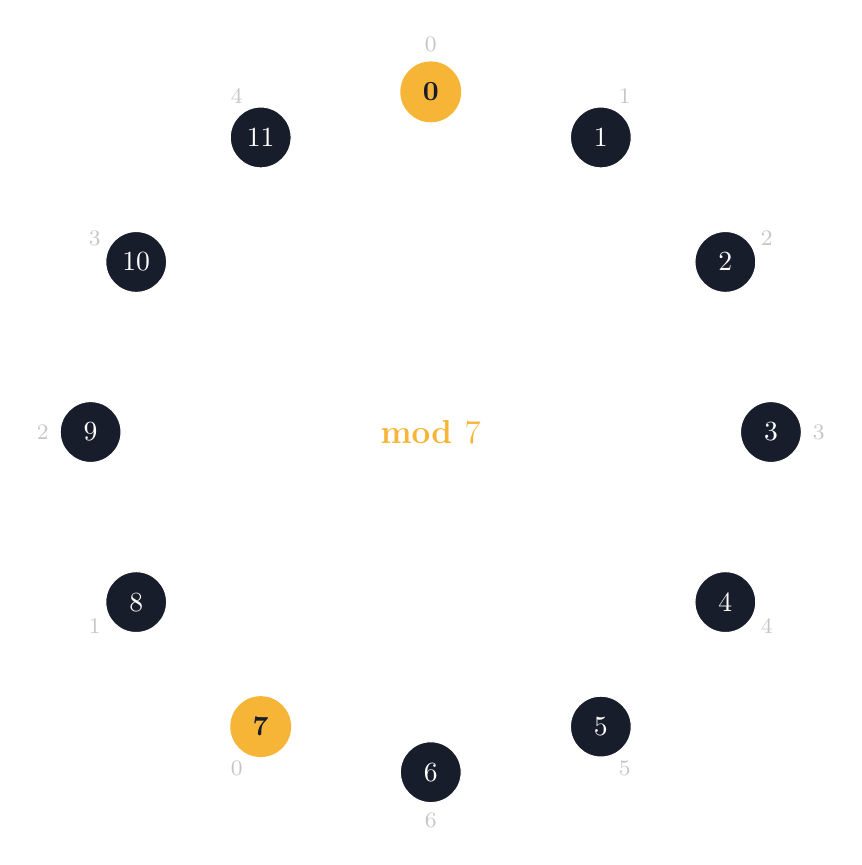
\begin{tikzpicture}[scale=1.35, text=teks]
  % lingkaran jam modulo 7: 12 titik, label = n mod 7
  \def\R{3.2}
  \draw[white, thick] (0,0) circle (\R);
  \foreach \i in {0,...,11} {
    \pgfmathsetmacro{\ang}{90 - \i*30}
    \pgfmathtruncatemacro{\sisa}{mod(\i,7)}
    \ifnum\sisa=0
      \node[circle, fill=aksen, text=latar, font=\bfseries,
            minimum size=22pt, inner sep=1pt] at (\ang:\R) {\i};
    \else
      \node[circle, fill=latar, draw=white, text=teks,
            minimum size=22pt, inner sep=1pt] at (\ang:\R) {\i};
    \fi
    \node[gray!45, font=\footnotesize] at (\ang:\R+0.45) {\sisa};
  }
  \node[text=aksen, font=\bfseries\large] at (0,0) {mod $7$};
\end{tikzpicture}
\end{document}
